\def\sectiontitle{Background}

\section{\sectiontitle}

%%%%%%%%%%%%%%%%%%%%%%%%%%%%%%%%%%%%%%%%%%%%%%%%%%%%%%%%%%%%%%%%%%%%%%%%%%%%%%%%
\def\slidetitle{Problem statement}

\subsection{\slidetitle}
\begin{frame}
  \frametitle{\sectiontitle}
  \framesubtitle{\slidetitle}

  Problem
  \begin{itemize}
    \item Lower the barriers for reusing trained AI models available in AI models repositories
  \end{itemize}

  Challenges
  \begin{itemize}
    \item Models are spread on lot of different repositories and formats
    \item For non-technical researchs, not trivial to setup and execute AI models
    \item Re-train models from scratch take lot of time and money
  \end{itemize}

  Motivations
  \begin{itemize}
    \item Accelerate application of AI models to scientific problems
    \item Save hours of computation time by reusing pre-trained models from diverse repositories
  \end{itemize}
\end{frame}

%%%%%%%%%%%%%%%%%%%%%%%%%%%%%%%%%%%%%%%%%%%%%%%%%%%%%%%%%%%%%%%%%%%%%%%%%%%%%%%%
\def\slidetitle{Related work}

\subsection{\slidetitle}
\begin{frame}
  \frametitle{\sectiontitle}
  \framesubtitle{\slidetitle}

  Already existing APIs or tools to download, inference (and train) AI models
  \begin{itemize}
    \item Transformers (Hugging Face API)*
    \item Cellpose API**
    \item BioImage.IO Core (Python libraries)
    \item SAM2 repository***
  \end{itemize}

  \bigskip
  \bigskip

  *https://aclanthology.org/2020.emnlp-demos.6/

  **https://www.biorxiv.org/content/10.1101/2020.02.02.931238v1

  ***https://arxiv.org/abs/2408.00714
\end{frame}

%%%%%%%%%%%%%%%%%%%%%%%%%%%%%%%%%%%%%%%%%%%%%%%%%%%%%%%%%%%%%%%%%%%%%%%%%%%%%%%%
\def\slidetitle{Our approach}

\subsection{\slidetitle}
\begin{frame}
  \frametitle{\sectiontitle}
  \framesubtitle{\slidetitle}

  \begin{minipage}[h!]{0.60\textwidth}

    Our approach
    \begin{itemize}
      \item Leverage WIPP
      \item Use AI model card
      \item Using existing API of AI repositories
    \end{itemize}

    \bigskip

    Web Image Processing Pipelines (WIPP)
    \begin{itemize}
      \item Purposes
      \begin{itemize}
        \item Measurements based on terabyte-sized images
        \item Algorithmic plugin platform
      \end{itemize}
      \item Goal
      \begin{itemize}
        \item Lower the bar to execute image analyses
      \end{itemize}
    \end{itemize}
  \end{minipage}\hfill
  \begin{minipage}[h!]{0.35\textwidth}
    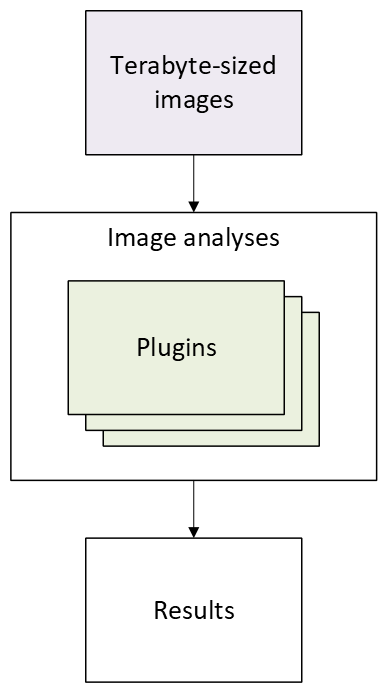
\includegraphics[scale=0.55]{./img/1_background/wipp.png}
  \end{minipage}
\end{frame}

%%%%%%%%%%%%%%%%%%%%%%%%%%%%%%%%%%%%%%%%%%%%%%%%%%%%%%%%%%%%%%%%%%%%%%%%%%%%%%%%
\def\slidetitle{Plugin concept}

\subsection{\slidetitle}
\begin{frame}
  \frametitle{\sectiontitle}
  \framesubtitle{\slidetitle}

  \begin{minipage}[h!]{0.40\textwidth}
    WIPP workflow
    \begin{itemize}
      \item Sequence of plugins
    \end{itemize}

    \bigskip

    WIPP plugin
    \begin{itemize}
      \item Piece of code taking inputs/outputs and executing code
    \end{itemize}
  \end{minipage}\hfill
  \begin{minipage}[h!]{0.55\textwidth}
    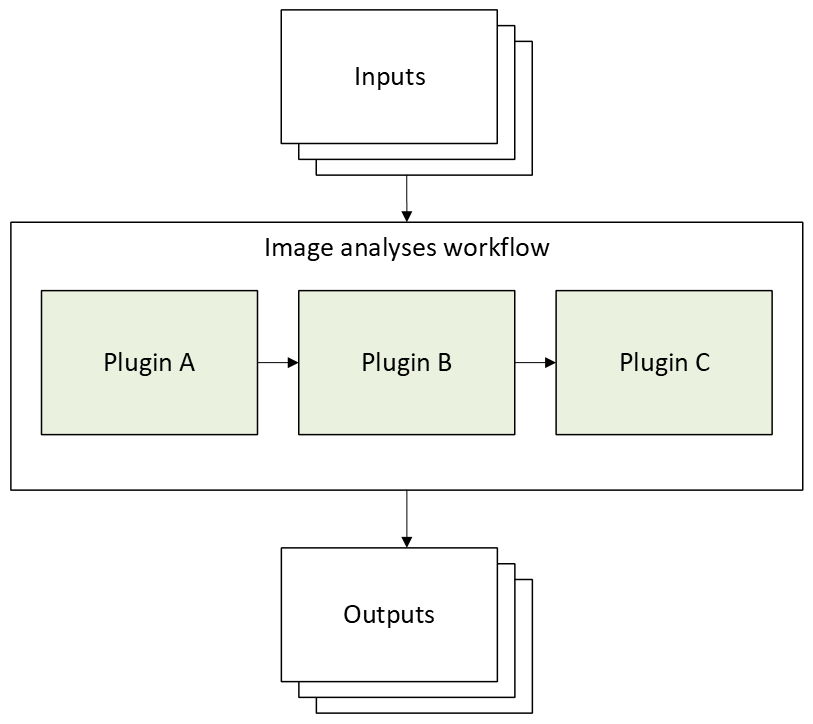
\includegraphics[scale=0.55]{./img/1_background/plugins.png}
  \end{minipage}
\end{frame}

%%%%%%%%%%%%%%%%%%%%%%%%%%%%%%%%%%%%%%%%%%%%%%%%%%%%%%%%%%%%%%%%%%%%%%%%%%%%%%%%
\def\slidetitle{AI model cards}

\subsection{\slidetitle}
\begin{frame}[containsverbatim]
  \frametitle{\sectiontitle}
  \framesubtitle{\slidetitle}

  Goal: Automatic documentation for AI models trained inside WIPP

  Work: Make AI model card proposal and development for integration

  \begin{listing}[H]
    \begin{minted}[frame=lines,framesep=2mm,baselinestretch=0.8,fontsize=\small,linenos]{java}
      public class AiModelCard {
        private String              version;
        private String              name;
        private Date                creationDate;
        private String              framework;
        private Map<String, String> trainingData;
        private Map<String, String> trainingParameters;
        [8 additional fields]
      }
    \end{minted}
    % \caption{AiModelCard.java}
  \end{listing}

  Feedback: Not relevant, AI users test directly, they don't read the documentation

\end{frame}

